\section{Moduler i en BMS}
For at kunne forklare de forskellige topologier er der nogle områder i en BMS der skal være styr på først. BMS'ens opgaver klares af flere moduler som ikke nødvendigvis behøver at hænge sammen. Afhængigt af den ønskede opsætning kan der være forskellige antal af de forskellige moduler. Disse moduler deles typisk ud på flere PCB'er hvis krævet, og er ofte delt op i tre forskellige: 

\subsubsection{Celleovervågningsmodul (CMU for engelsk "Cell monitoring unit")}
Dette modul er direkte forbundet til hver enkel celle. Her overvåges spænding, temperatur og andre vitale dele af cellens parametre, samt at der er her balanceringen finder sted. 

\subsubsection{Modulstyring (MMU for engelsk "Module manangement unit")}
MMU'en styrer en gruppe af de førnævnte CMU'er, og dette modul gør det derfor muligt at balancere cellerne i forhold til hinanden. 

\subsubsection{Batteripakkestyring (PMU for engelsk "Pack management unit")}
Batteripakkestyringen er det overordnede modul. Her styres MMU'erne, men samtidig holdes der også styr på hele pakkens spænding og strøm. Det er også her at sikkerhedsforanstaltningerne sidder, såsom kortslutningsbeskyttelse samt over- og afladningsbeskyttelse. Kommunikation med andre eksterne systemer foregår også her. 

\section{Centraliseret system}
I et centraliseret system er alle tre slags moduler kombineret til én enhed. Derfor er alle cellerne koblet direkte til systemet med ledninger, og alle BMS'ens funktioner er tilgængelige uden ekstra moduler. \\

Et centraliseret system er den mest økonomiske, men mindst udvidelige måde at udvikle en BMS på. Der er også ret mange ledninger, da der skal gå ledninger ud til hver enkelt celle. En centraliseret BMS er også forholdsvis simpel at opbygge uden alt for mange kompromisser. På grund af dens simple opbygning er den mest egnet til batteripakker med få antal celler. Derfor gør det den ideel til f.eks. el-cykler eller andre mindre elektriske "gadgets", og mindre ideel til f.eks. el-biler. På figur \ref{fig:centralized_BMS} ses opbygningen af en centraliseret BMS. \\

\begin{figure}[h]
	\centering
	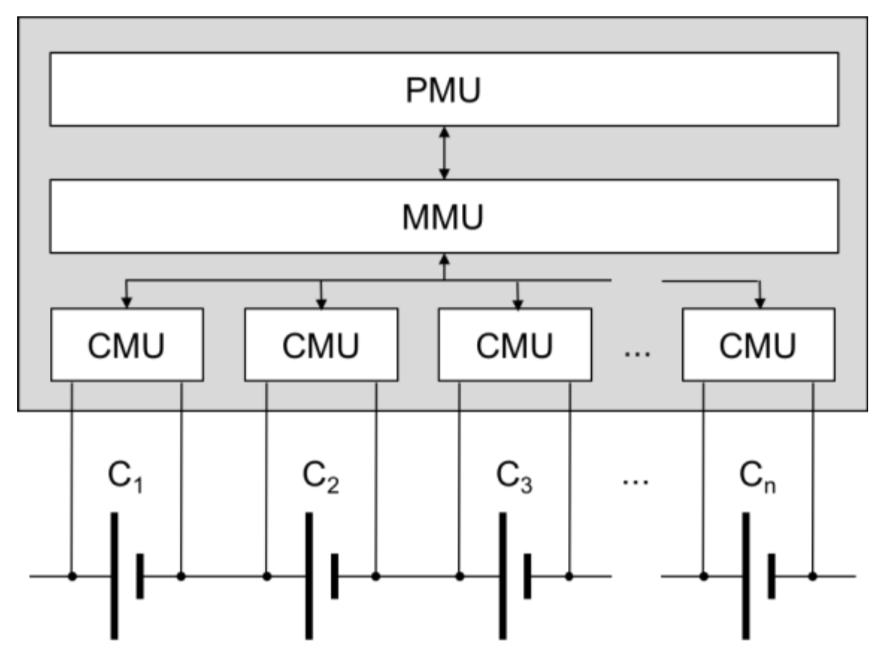
\includegraphics[width=8cm]{billeder/centralized.png}
	\caption{En centraliseret BMS}
	\label{fig:centralized_BMS}
\end{figure}

\section{Distribueret system}
I et distribueret system foretages alle målinger på den enkelte celle og kommunikerer sin status til en master enhed. Hver celle er udstyret med sin egen dedikerede CMU og MMU. De enkelte MMU'er kan kommunikere med hinanden afhængig af behov. \\

\begin{figure}[h]
	\centering
	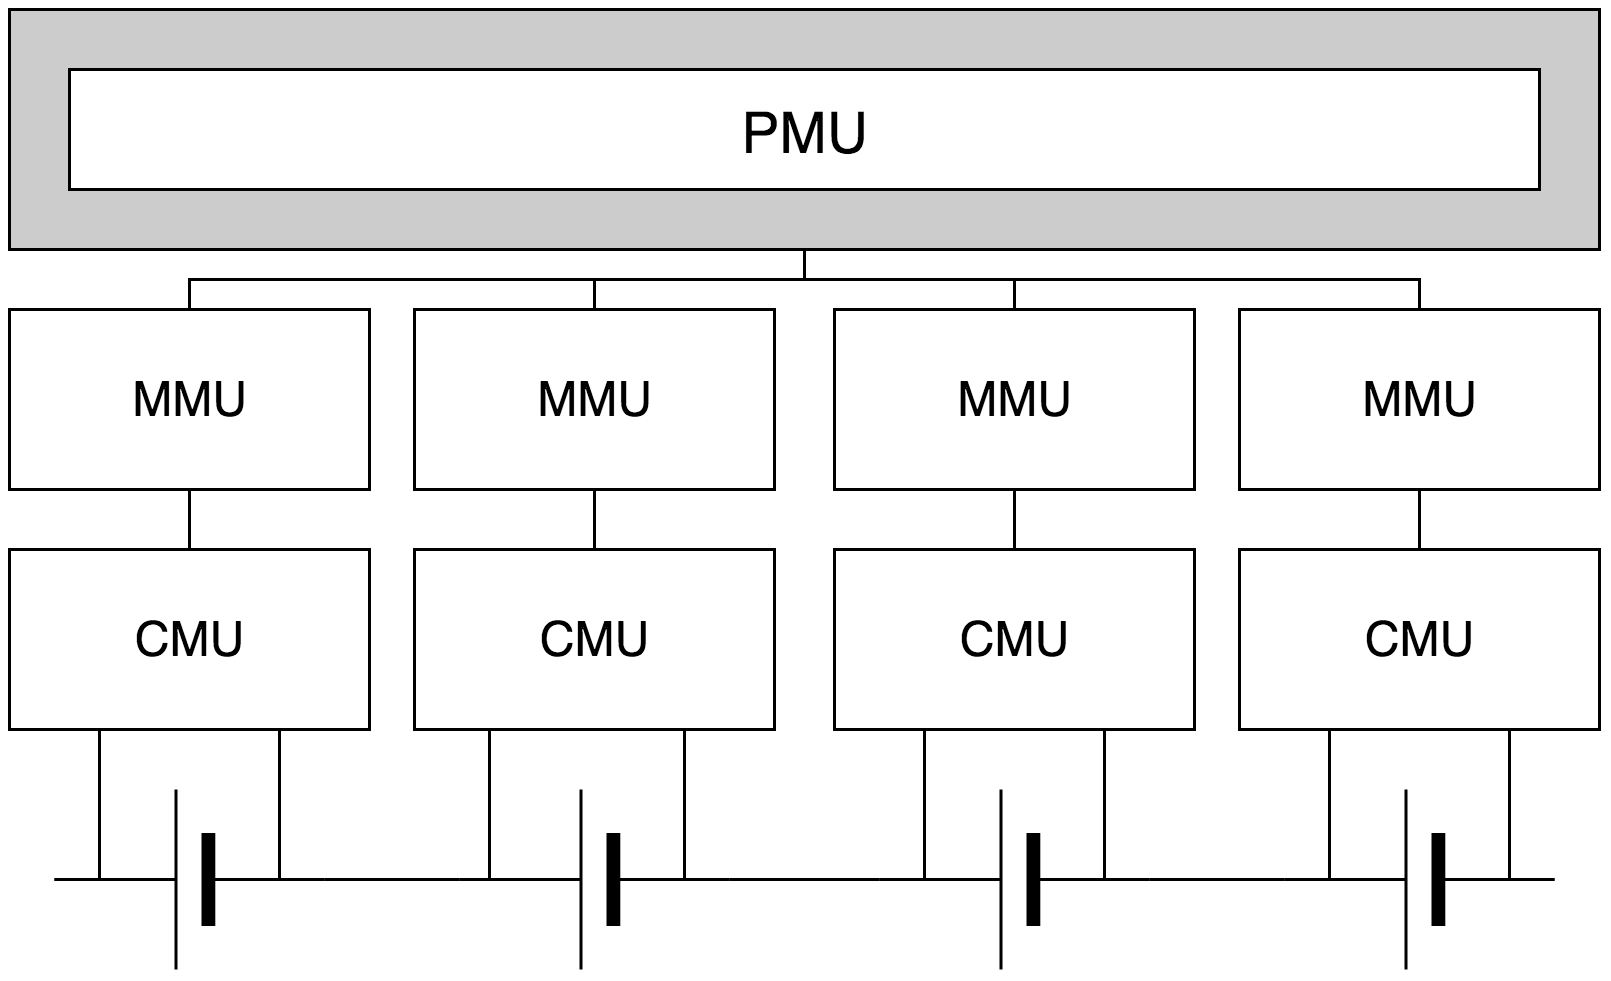
\includegraphics[width=8cm]{billeder/distributed.png}
	\caption{En distribueret BMS}
	\label{fig:distributed_BMS}
\end{figure}

Fordelen ved denne topologi er at designet er "gentageligt" og pålideligt. Ulempen er dog, at den kræver et højt antal slave enheder, som kan give problemer rent monteringsmæssigt.

\section{Modulær system}
Den modulære topologi er en blanding af den centraliserede og distribuerede. Her er opdeles MMU'en i flere blokke der hver har ansvaret for flere celler. Har man derfor en stor batteripakke på 48 celler, kan én MMU f.eks. holde styr på 12 celler og CMU'er, og så har man 4 MMU'er. Disse MMU'er er så stadig forbundet til én PMU, som holder styr på det hele og sørger for kommunikation i mellem modulerne. \\

\begin{figure}[h]
	\centering
	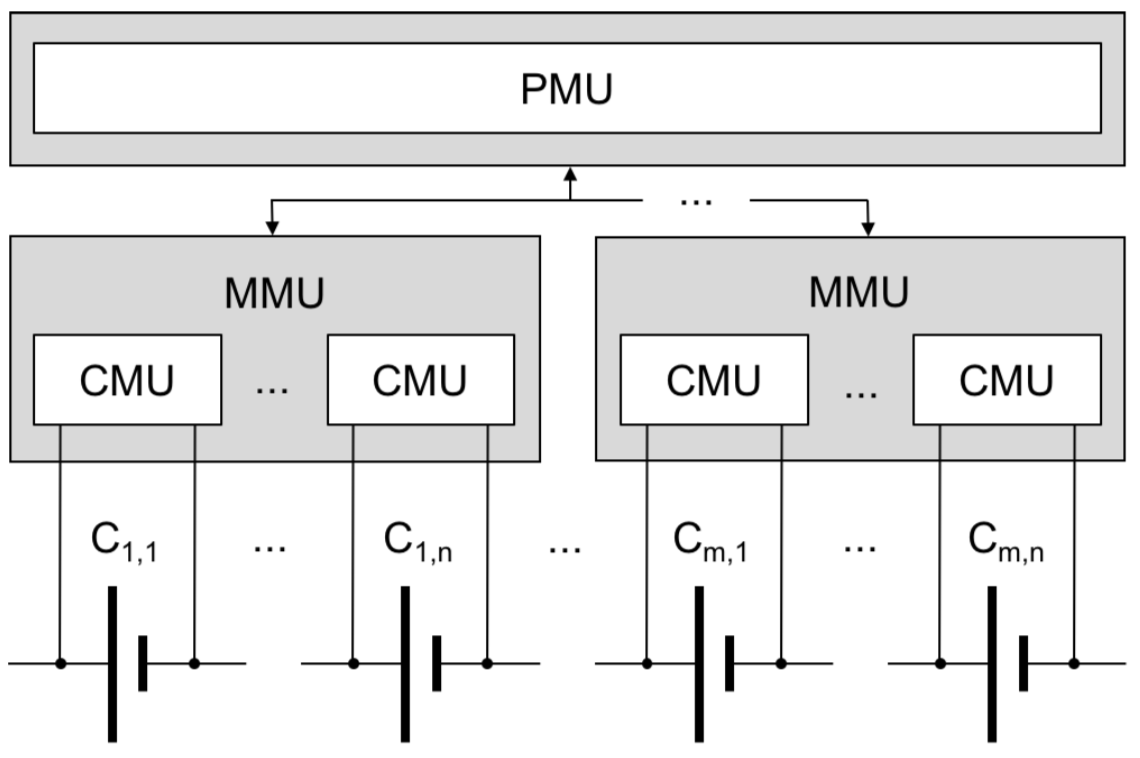
\includegraphics[width=8cm]{billeder/modular.png}
	\caption{En modulær BMS}
	\label{fig:modular_BMS}
\end{figure}

Denne topologi egner sig til systemer hvor cellerne nødvendigvis ikke kan være lige ved siden af hinanden, men opbevares i grupper, som f.eks. forskellige steder i en el-bil.

\section{Valg af topologi}
Af de tre forskellige topologier er det blevet besluttet at vælge det centraliserede system hovedsageligt pga. dets enkelthed. Til projektets formål er det ikke nødvendigt at kunne dele batteripakken op i grupper, og det er heller ikke nødvendigt at styresystemet sidder langt væk fra cellerne. Her skal systemet monteres sammen med cellerne hvilket også giver fordele ved f.eks. temperaturmåling. Da batteripakken i dette system ikke har mere end 4 celler i serie er det også det oplagte valg. 